\documentclass[geometry_main]{subfiles}

\begin{document}

\setcounter{chapter}{3}

\chapter{小技集}

この章では,これまでに登場した種々の定理の証明に使われる数学の小技を紹介する.

\section{集合と写像の関係}

\begin{mylem}[label=lem:sets,breakable]{集合論の小定理集}
	$f \colon X \to Y$ を写像とする.また,$\Lambda,\, M$ を任意の添字集合とし, $U,\, U_\lambda \subset X\; (\lambda \in \Lambda)$,$V,\, V_\mu \subset Y\; (\mu \in M)$ とする.
	\begin{enumerate}
		\item 
		\begin{align}
			f\Biggl(\bigcup_{\lambda \in \Lambda} U_\lambda \Biggr) = \bigcup_{\lambda \in \Lambda} f(U_\lambda)
		\end{align}
		\item 
		\begin{align}
			f\Biggl(\bigcap_{\lambda \in \Lambda} U_\lambda \Biggr) \subset \bigcap_{\lambda \in \Lambda} f(U_\lambda)
		\end{align}
		\item 
		\begin{align}
			f^{-1}\Biggl(\bigcup_{\mu \in M} V_\mu \Biggr) = \bigcup_{\mu \in M} f^{-1}(V_\mu)
		\end{align}
		\item \begin{align}
			f^{-1}\Biggl(\bigcap_{\mu \in M} V_\mu \Biggr) = \bigcap_{\mu \in M} f^{-1}(V_\mu)
		\end{align}
		\item \begin{align}
			f^{-1}\bigl(V^c \bigr) = \bigl(f^{-1}(V)\bigr)^c
		\end{align}
		\item \begin{align}
			f \bigl( f^{-1} (V)\bigr) = V \cap f(X)
		\end{align}
		\item \begin{align}
			f^{-1}\bigl( f (U)\bigr) \supset U
		\end{align}
		\item \begin{align}
			f(X) \setminus f(U) \subset f(U^c)
		\end{align}
        \item 以下の4つは互いに同値である:
        \begin{enumerate}
            \item 任意の集合族 $\bigl\{\, U_\lambda \, \bigr\}_{\lambda \in \Lambda} \subset 2^X$ に対して
            \begin{align}
                f \Biggl(\bigcap_{\lambda \in \Lambda} U_\lambda\Biggr) = \bigcap_{\lambda \in \Lambda} f(U_\lambda)
            \end{align}
            \item \begin{align}
                \forall U \in 2^X,\; f^{-1}\bigl( f(U) \bigr) = U
            \end{align}
            \item \begin{align}
                \forall U \in 2^X,\; f(X) \setminus f(U) = f(U^c)
            \end{align}
            \item $f$ は単射
        \end{enumerate}
        \item 以下の2つは同値である:
        \begin{enumerate}
            \item 
            \begin{align}
                \forall V \in 2^Y,\; f \bigl( f^{-1}(V) \bigr) = V
            \end{align}
            \item $f$ は全射
        \end{enumerate}
	\end{enumerate}
\end{mylem}

\begin{proof}
    \begin{enumerate}
        \item $\bm{(\subset):}$
        \begin{align}
            y \in f \Biggl(\bigcup_{\lambda \in \Lambda} U_\lambda\Biggr)\quad \Longrightarrow\quad \exists x \in \bigcup_{\lambda \in \Lambda} U_\lambda,\; f(x) = y\quad \Longrightarrow\quad \exists \alpha \in \Lambda,\; y \in f(U_\alpha) \subset \bigcup_{\lambda \in \Lambda} f(U_\lambda).
        \end{align}
        $\bm{(\supset):}$
        \begin{align}
            y \in \bigcup_{\lambda \in \Lambda} f(U_\lambda) \quad \Longrightarrow\quad \exists \alpha \in \Lambda,\; y \in f(U_\alpha)\quad \Longrightarrow \quad y \in f\Biggl(\bigcup_{\lambda \in \Lambda} U_\lambda\Biggr)
        \end{align}
        \item 
        \begin{align}
            y \in f\Biggl(\bigcap_{\lambda \in \Lambda} U_\lambda\Biggr) \quad \Longleftrightarrow \quad \exists x \in \bigcap_{\lambda \in \Lambda} U_\lambda,\; y = f(x)  \quad \textcolor{red}{\Longrightarrow} \quad  \forall \alpha \in \Lambda,\; y \in f(U_\alpha) \quad \Longleftrightarrow \quad \bigcap_{\lambda \in \Lambda} f(U_\lambda).
        \end{align}
        \item $\bm{(\subset):}$
        \begin{align}
            x \in f^{-1} \Biggl(\bigcup_{\mu \in M} V_\mu\Biggr)\quad \Longrightarrow\quad f(x) \in \bigcup_{\mu \in M} V_\mu \quad \Longrightarrow\quad \exists \alpha \in M,\; f(x) \in V_\alpha \subset \bigcup_{\mu \in M} f^{-1}(V_\mu).
        \end{align}
        $\bm{(\supset):}$
        \begin{align}
            x \in \bigcup_{\mu \in M} f^{-1} \bigl(V_\mu\bigr)\quad \Longrightarrow\quad \exists \alpha \in M,\; x \in f^{-1}(V_\alpha) \quad \Longrightarrow\quad x \in f^{-1} \Biggl(\bigcup_{\mu \in M} f^{-1}(V_\mu)\Biggr).
        \end{align}
        \item $\bm{(\subset):}$
        \begin{align}
            x \in f^{-1} \Biggl(\bigcap_{\mu \in M} V_\mu\Biggr)\quad \Longrightarrow\quad f(x) \in \bigcap_{\mu \in M} V_\mu \quad \Longrightarrow\quad \forall \alpha \in M,\; f(x) \in V_\mu\quad \Longrightarrow\quad x \in \bigcap_{\mu \in M} f^{-1}(V_\mu).
        \end{align}
        $\bm{(\supset):}$
        \begin{align}
            x \in \bigcap_{\mu \in M} f^{-1} \Biggl(V_\mu\Biggr)\quad \Longrightarrow\quad \forall \alpha \in M,\; f(x) \in V_\alpha \quad \Longrightarrow\quad f(x) \in \bigcap_{\mu \in M} V_\mu \quad \Longrightarrow\quad x \in f^{-1} \Biggl(\bigcap_{\mu \in M} V_\mu\Biggr).
        \end{align}
        \item
        \begin{align}
            x \in f^{-1} \bigl( Y \setminus V \bigr) \quad \Longleftrightarrow\quad f(x) \in Y \AND f(x) \notin V \quad \Longleftrightarrow\quad x \in f^{-1}(Y) \setminus f^{-1}(V)
        \end{align}
        \item 
        \begin{align}
            y \in f \bigl( f^{-1}(V) \bigr)  \quad &\Longleftrightarrow\quad \exists x \in f^{-1}(V),\; y = f(x) \\
            &\Longleftrightarrow\quad \exists x \in U,\; f(x) \in V \AND y = f(x) \\
            &\Longleftrightarrow\quad y \in V \AND y \in f(X)
        \end{align}
        \item 
        \begin{align}
            x \in U \quad \textcolor{red}{\Longrightarrow}\quad f(x) \in f(U) \quad \Longleftrightarrow\quad x \in f^{-1}\bigl( f(U) \bigr) 
        \end{align}
        \item 
        \begin{align}
            y \in f(X) \AND y \notin f(U) \quad &\Longleftrightarrow\quad \bigl(\, \exists x \in X,\; y = f(x) \, \bigr) \AND \bigl(\, \forall u \in U,\; y \neq f(u)\, \bigr) \\
            &\textcolor{red}{\Longrightarrow}\quad \exists x \in X \setminus U,\; y = f(x) \label{eq:apD-4-1-1}\\
            &\Longleftrightarrow\quad y \in f(U^c)
        \end{align}
        \item $\bm{(d) \; \Longrightarrow\; (c):}$ 
        
         $f$ が単射なら (8) の証明中の命題\eqref{eq:apD-4-1-1}が
        \begin{align}
            \exists !\, x \in X \setminus U,\; y = f(x)
        \end{align}
        になり\footnote{$\exists !$ は「ただ一つ存在する」の意味である.},$\textcolor{red}{\Longrightarrow}$ の逆も成り立つ.

        $\bm{(c) \; \Longrightarrow\; (b):}$ 
        
         仮定より,$\forall x \in X$ に対して
        \begin{align}
            f(x) \in f(U) = f \bigl( (X \setminus U)^c \bigr) \quad \Longrightarrow \quad f(x) \notin f(X \setminus U) \quad \Longrightarrow \quad x \in U
        \end{align}
        が成り立つ.i.e. (7) の証明において $\textcolor{red}{\Longrightarrow}$ の逆も成り立つ.

        $\bm{(b) \; \Longrightarrow\; (a):}$
        \begin{align}
            y \in \bigcap_{\lambda \in \Lambda} f(U_\lambda) \quad \Longleftrightarrow \quad \exists x \in X,\; \alpha \in \Lambda,\, \exists x_\alpha \in U_\alpha,\; y = f(x_\alpha).
        \end{align}
        ここで $\forall \alpha,\, \beta \in \Lambda$ をとり,一点集合 $\{ x_\alpha \},\; \{ x_\beta \} \in 2^X$ に対して (b) を使うと
        \begin{align}
            \{ x_\alpha \} = f^{-1} \bigl( f(\{ x_\alpha \}) \bigr) = f^{-1}(\{ y \}) = f^{-1} \bigl( f(\{ x_\beta \}) \bigr) = \{ x_\beta \}
        \end{align}
        がわかる.i.e. $\forall \alpha,\, \beta \in \Lambda,\; x_\alpha = x_\beta.$ ゆえに (2) の証明における $\textcolor{red}{\Longrightarrow}$ の逆も成り立つ.

        $\bm{(a) \; \Longrightarrow\; (d):}$ 
        
         $f(x_1) = f(x_2) = y$ とする.(a) から
        \begin{align}
            f(\{x_1\} \cap \{x_2\}) = f(\{x_1\}) \cap f(\{x_2\}) = \{y\} \neq \emptyset
        \end{align}
        だから $\{x_1\} \cap \{x_2\} \neq \emptyset$ でなくてはならない.i.e. $x_1 = x_2.$
        \item (6) より,$\forall V \in 2^Y$ に対して
        \begin{align}
            \label{eq.apD-4-1-2}
            f \bigl( f^{-1}(V) \bigr) = V \quad \Longleftrightarrow \quad V = V \cap f(X) \quad \Longleftrightarrow \quad V \subset f(X)
        \end{align}
        が成り立つ.
        
        $\bm{(\Longrightarrow):}$ 

         仮定 (a) と命題\eqref{eq.apD-4-1-2}より $Y \subset f(X).$ 一方 $f$ が写像であることから $f(X) \subset Y$ であり,$f(X) = Y$ がわかる.
        
        $\bm{(\Longleftarrow):}$
        
         仮定 (b) より $f(X) = Y$ であるから,$\forall V \in 2^Y$ に対して $V \subset f(X)$ が成り立つ.従って命題\eqref{eq.apD-4-1-2}を使うことができて,(a) が成立する.
    \end{enumerate}
\end{proof}

\begin{mylem}[label=lem:finite-bijection]{有限集合上の単射と全射}
    $A,\, B$ が有限集合で,かつ $\abs{A} = \abs{B}$ ならば次の (1), (2) が成り立つ:
    \begin{enumerate}
        \item $A \subset B \IMP A=B$
        \item $f \colon A \to B$ が写像ならば,$f$ が単射であることと $f$ が全射であることは同値である.
    \end{enumerate}
\end{mylem}

\begin{proof}
    \begin{enumerate}
        \item 仮定より $B = A \sqcup (B \setminus A)$ である.ゆえに $\abs{B} = \abs{A} + \abs{B \setminus A}$ だが,仮定より $\abs{A} = \abs{B}$ なので $\abs{B \setminus A} = 0.$ i.e. $B \setminus A = \emptyset$ である.
        \item $\bm{(\Longrightarrow):}$
        
         $f$ を単射とする.このとき仮定より $\abs{f(A)} = \abs{A} = \abs{B}$ である.$f(A) \subset B$ でもあるから,(1) より $f(A) = B$ がわかる.

        $\bm{(\Longleftarrow):}$

         $f$ を全射とする.$\forall b \in B$ に対して,$a_b \in A$ であって $f(a_b) = b$ を充たすものを一つずつ選んでおき,$A$ の部分集合 $C$ を
        \begin{align}
            C \coloneqq \bigl\{\, a_b \in A \bigm| b \in B\,\bigr\} \subset A
        \end{align}
        として定める.
        
         $\forall b_1,\, b_2 \in B$ に対して,$b_1 \neq b_2 \AND a_{b_1} = a_{b_2}$ を仮定すると $b_1 = f(a_{b_1}) = f(a_{b_2}) = b_2$ となり矛盾である.よって背理法から $b_1 \neq b_2 \IMP a_{b_1} \neq a_{b_2}$ であり,仮定から $\abs{C} = \abs{B} = \abs{A}$ とわかる.$C \subset A$ でもあるから (1) が使えて $C = A.$ これは $\forall b \in B$ に対して $f^{-1}(\{b\}) = \{ a_b \}$(一点集合)であることを意味するから,$f$ は単射である.
    \end{enumerate}
\end{proof}


\section{$C^\infty$ 関数の構成}

$\mathbb{R}^n$ において原点を中心とする半径 $r$ の開円板を $D(r)$ と書く.

$C^\infty$ 級関数 $h \colon \mathbb{R} \to \mathbb{R}$ を次のように定義する:
\begin{align}
	h(x) \coloneqq
	\begin{cases}
		e^{-1/x} & \colon x > 0 \\
		0 & \colon x \le 0
	\end{cases}
\end{align}
この $h$ を使って \cinfty 関数 $b \colon \mathbb{R}^n \to \mathbb{R}$ を次のように定義する:
\begin{align}
	b(x) \coloneqq \frac{h(4 - \abs{\vb*{x}}^2)}{h(4 - \abs{\vb*{x}}^2) + h(\abs{\vb*{x}}^2 - 1)}
\end{align}
この \cinfty 関数は以下の条件を充たす:
\begin{align}
	b(x) = \label{eq:apD-bump}
	\begin{cases}
		1 & \colon x \in \overline{D(1)} \\
		0 & \colon x \notin D(2)
	\end{cases}
\end{align}
実際,$b(x)$ をプロットしてみると図\ref{fig:apD-bump}のようになる.

\begin{figure}[H]
    \centering
    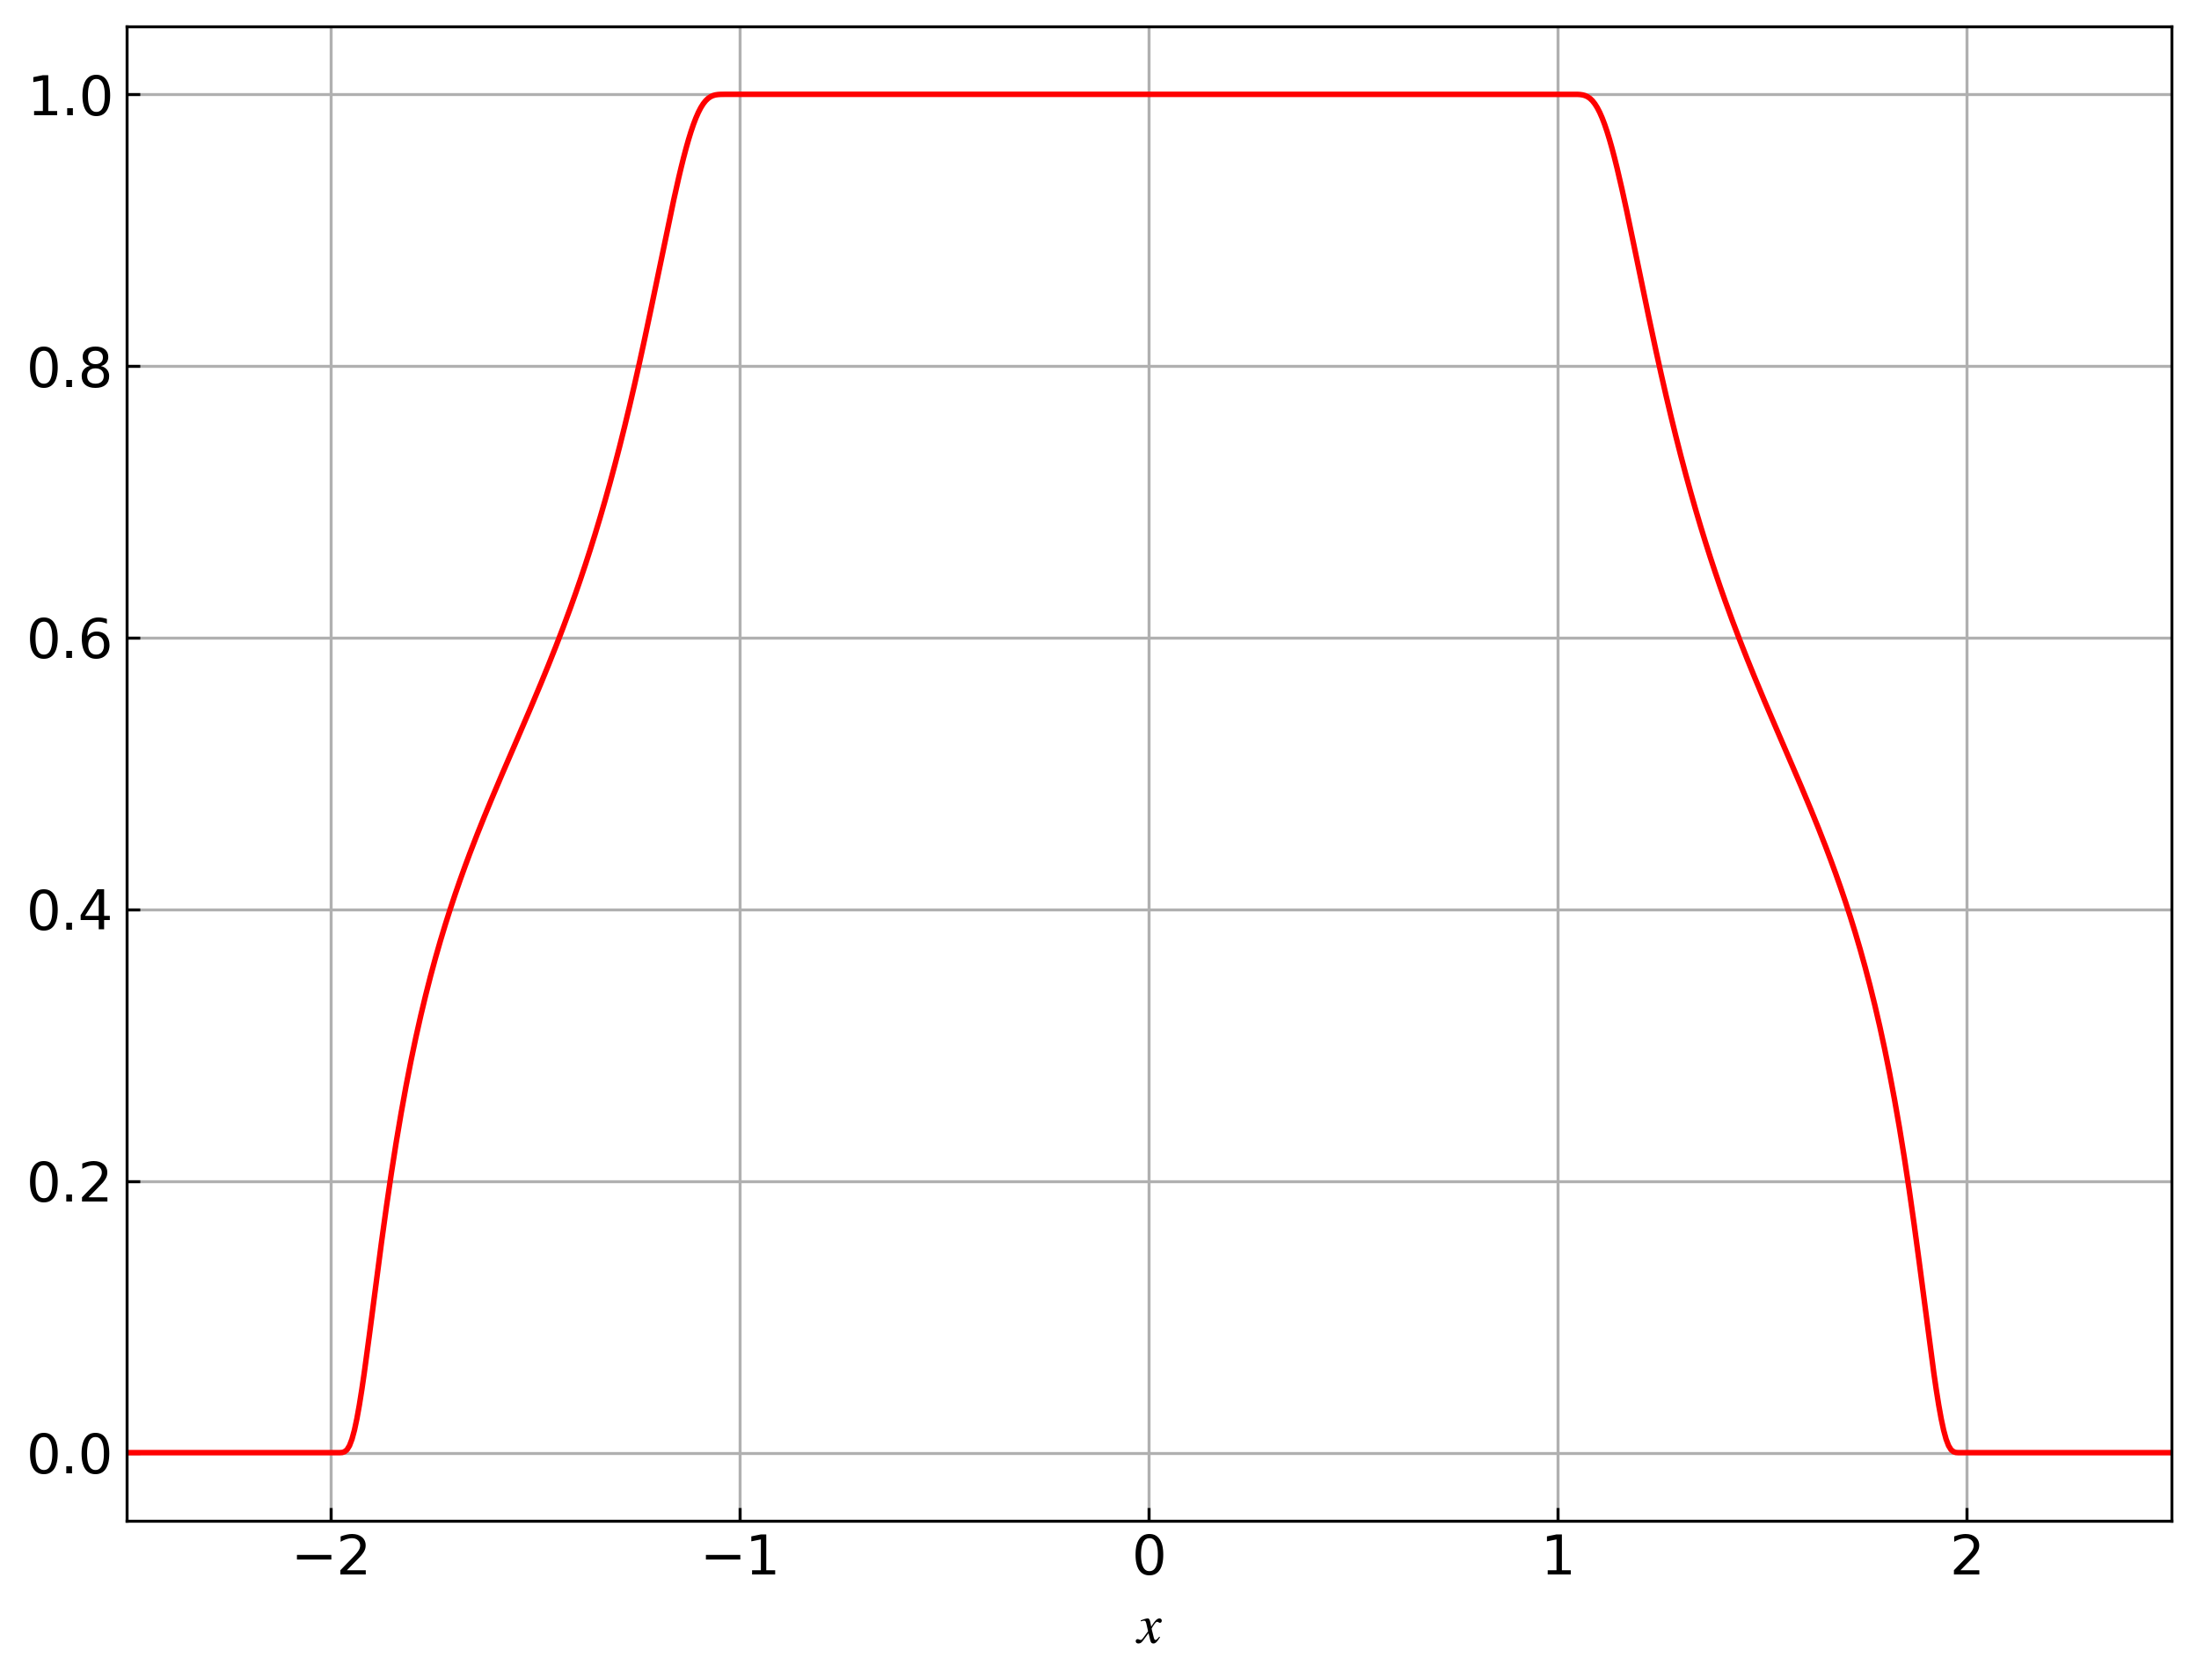
\includegraphics[scale=0.45]{./figs/fig-apD_bump.png}
    \caption{$b(x)$ のグラフ.$x \in [-1,\, 1]$ において $b(x) = 1$ であり,$\abs{x} \ge 2$ に対して $b(x) = 0$ となっている様子が確認できる.}
    \label{fig:apD-bump}
\end{figure}%

\begin{mylem}[label=gen_cinfty]{\cinfty 関数の拡張}
	$M$ を \cinfty 多様体とする.点 $p \in M$ の開近傍 $U$ と $U$ 上の\cinfty 関数 $f \colon U \to \mathbb{R}$ を任意にとる.

	このとき,$\overline{V} \subset U$ となる $p$ の開近傍 $V$ と,$M$ 全体で定義された\cinfty 関数 $\tilde{f} \colon M \to \mathbb{R}$ で
	\begin{align}
		\tilde{f}(q) =
		\begin{cases}
			f(q) & \colon q \in V \\
			0 &\colon q \notin U
		\end{cases}
	\end{align}
	を充たすものが存在する.
\end{mylem}

\begin{proof}
    点 $p$ を含むチャート $(W,\, \varphi)$ であって,$W \subset U$ かつ $\varphi(p) = 0,\; \varphi(W) \supset D(3)$ を充たすものをとる\footnote{このようなチャートは,$\mathbb{R}^n$ の原点を中心とする相似拡大を施すことでいつでも作ることができる.}.

    式\eqref{eq:apD-bump}の関数 $b$ を使って \cinfty 関数 $\tilde{b} W \to \mathbb{R}$ を $\tilde{b} \coloneqq b \circ \varphi$ と定義する.その構成から明らかに $\varphi^{-1}(D(1))$ の外側で $\tilde{b}$ は $0$ になる.故に $M\setminus W$ においては常に $0$ と定義して $\tilde{b}$ の定義域を拡張することで, $\tilde{b} \in \cinftyf{M}$ とすることができる.
    
    ここで $V \coloneqq \varphi^{-1}(D(1))$ とおくと $V$ は $p$ の開近傍になるが,明らかに $\overline{V} \subset U$ であり,かつ $V$ 上で $\tilde{b}$ は常に $1$ である.このとき $M$ 上の関数 $\tilde{f}$
    \begin{align}
        \tilde{f}(q) \coloneqq
		\begin{cases}
			\tilde{b}(q) f(q) & \colon q \in V \\
			0 &\colon q \notin U
		\end{cases}
    \end{align}
    は\cinfty 級であり,求める性質を充している.
\end{proof}

\end{document}